% \begin{frame}{\large Research Objective: Rectification with Min. Topological Changes}
% \begin{figure}
% \centering
% 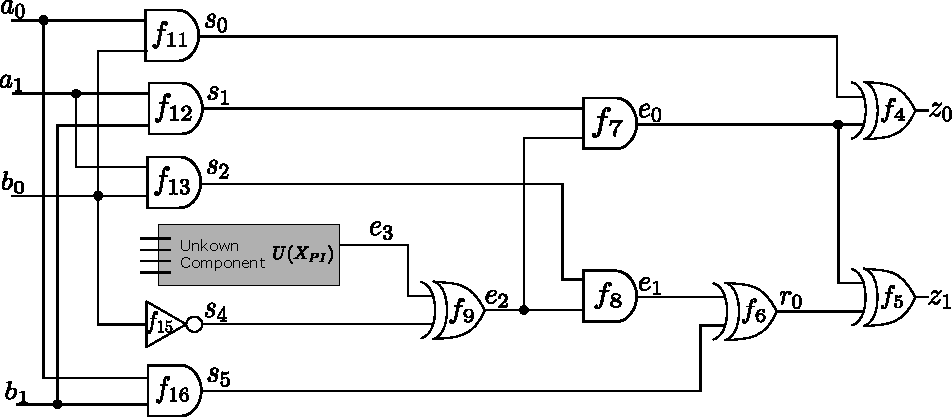
\includegraphics[scale=0.5]{mas_redundant_U.pdf}
% \end{figure}
% \bi
% 	\item In current formulation $U$ function of $X_{PI}$
% 	\item Disadvantage if net closer to PO
% 	\bi
% 		\item Re-synthesize significant portion of circuit
% 	\ei
% \ei
% \end{frame}

% \begin{frame}{\large Research Objective: Rectification with Min. Topological Changes}
% \begin{figure}
% \centering
% 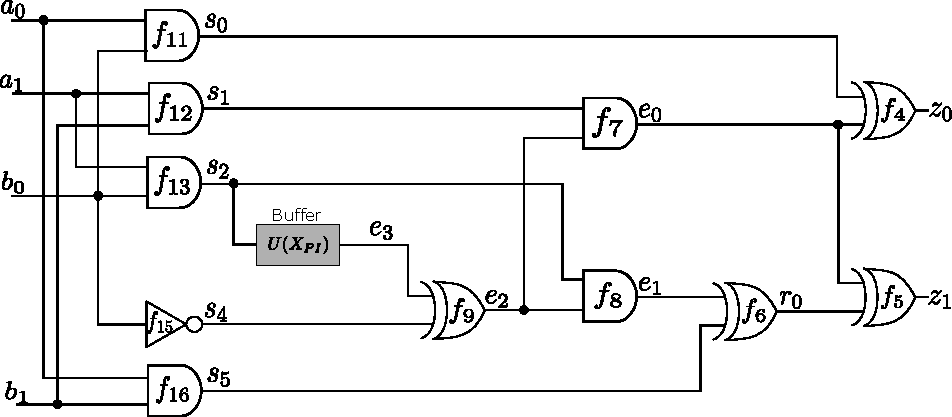
\includegraphics[scale=0.5]{mas_redundant_U_rewire.pdf}
% \end{figure}
% \bi
% 	\item Objective: Obtain $U$ in internal variables
% 	\bi
% 		\item Reuse already implemented logic
% 		\item Minimum (minimal) changes to the existing circuit
% 	\ei
% 	\item Approach: Different term orders for rectification formulation
% 	\bi
% 		\item Expensive GB computations in reduction procedures as RTTO $>$ is modified
% 	\ei
% \ei
% \end{frame}


% \begin{frame}{\large Research Objective: Integer arithmetic circuits}
% \begin{figure}[H]
%     \centering
%     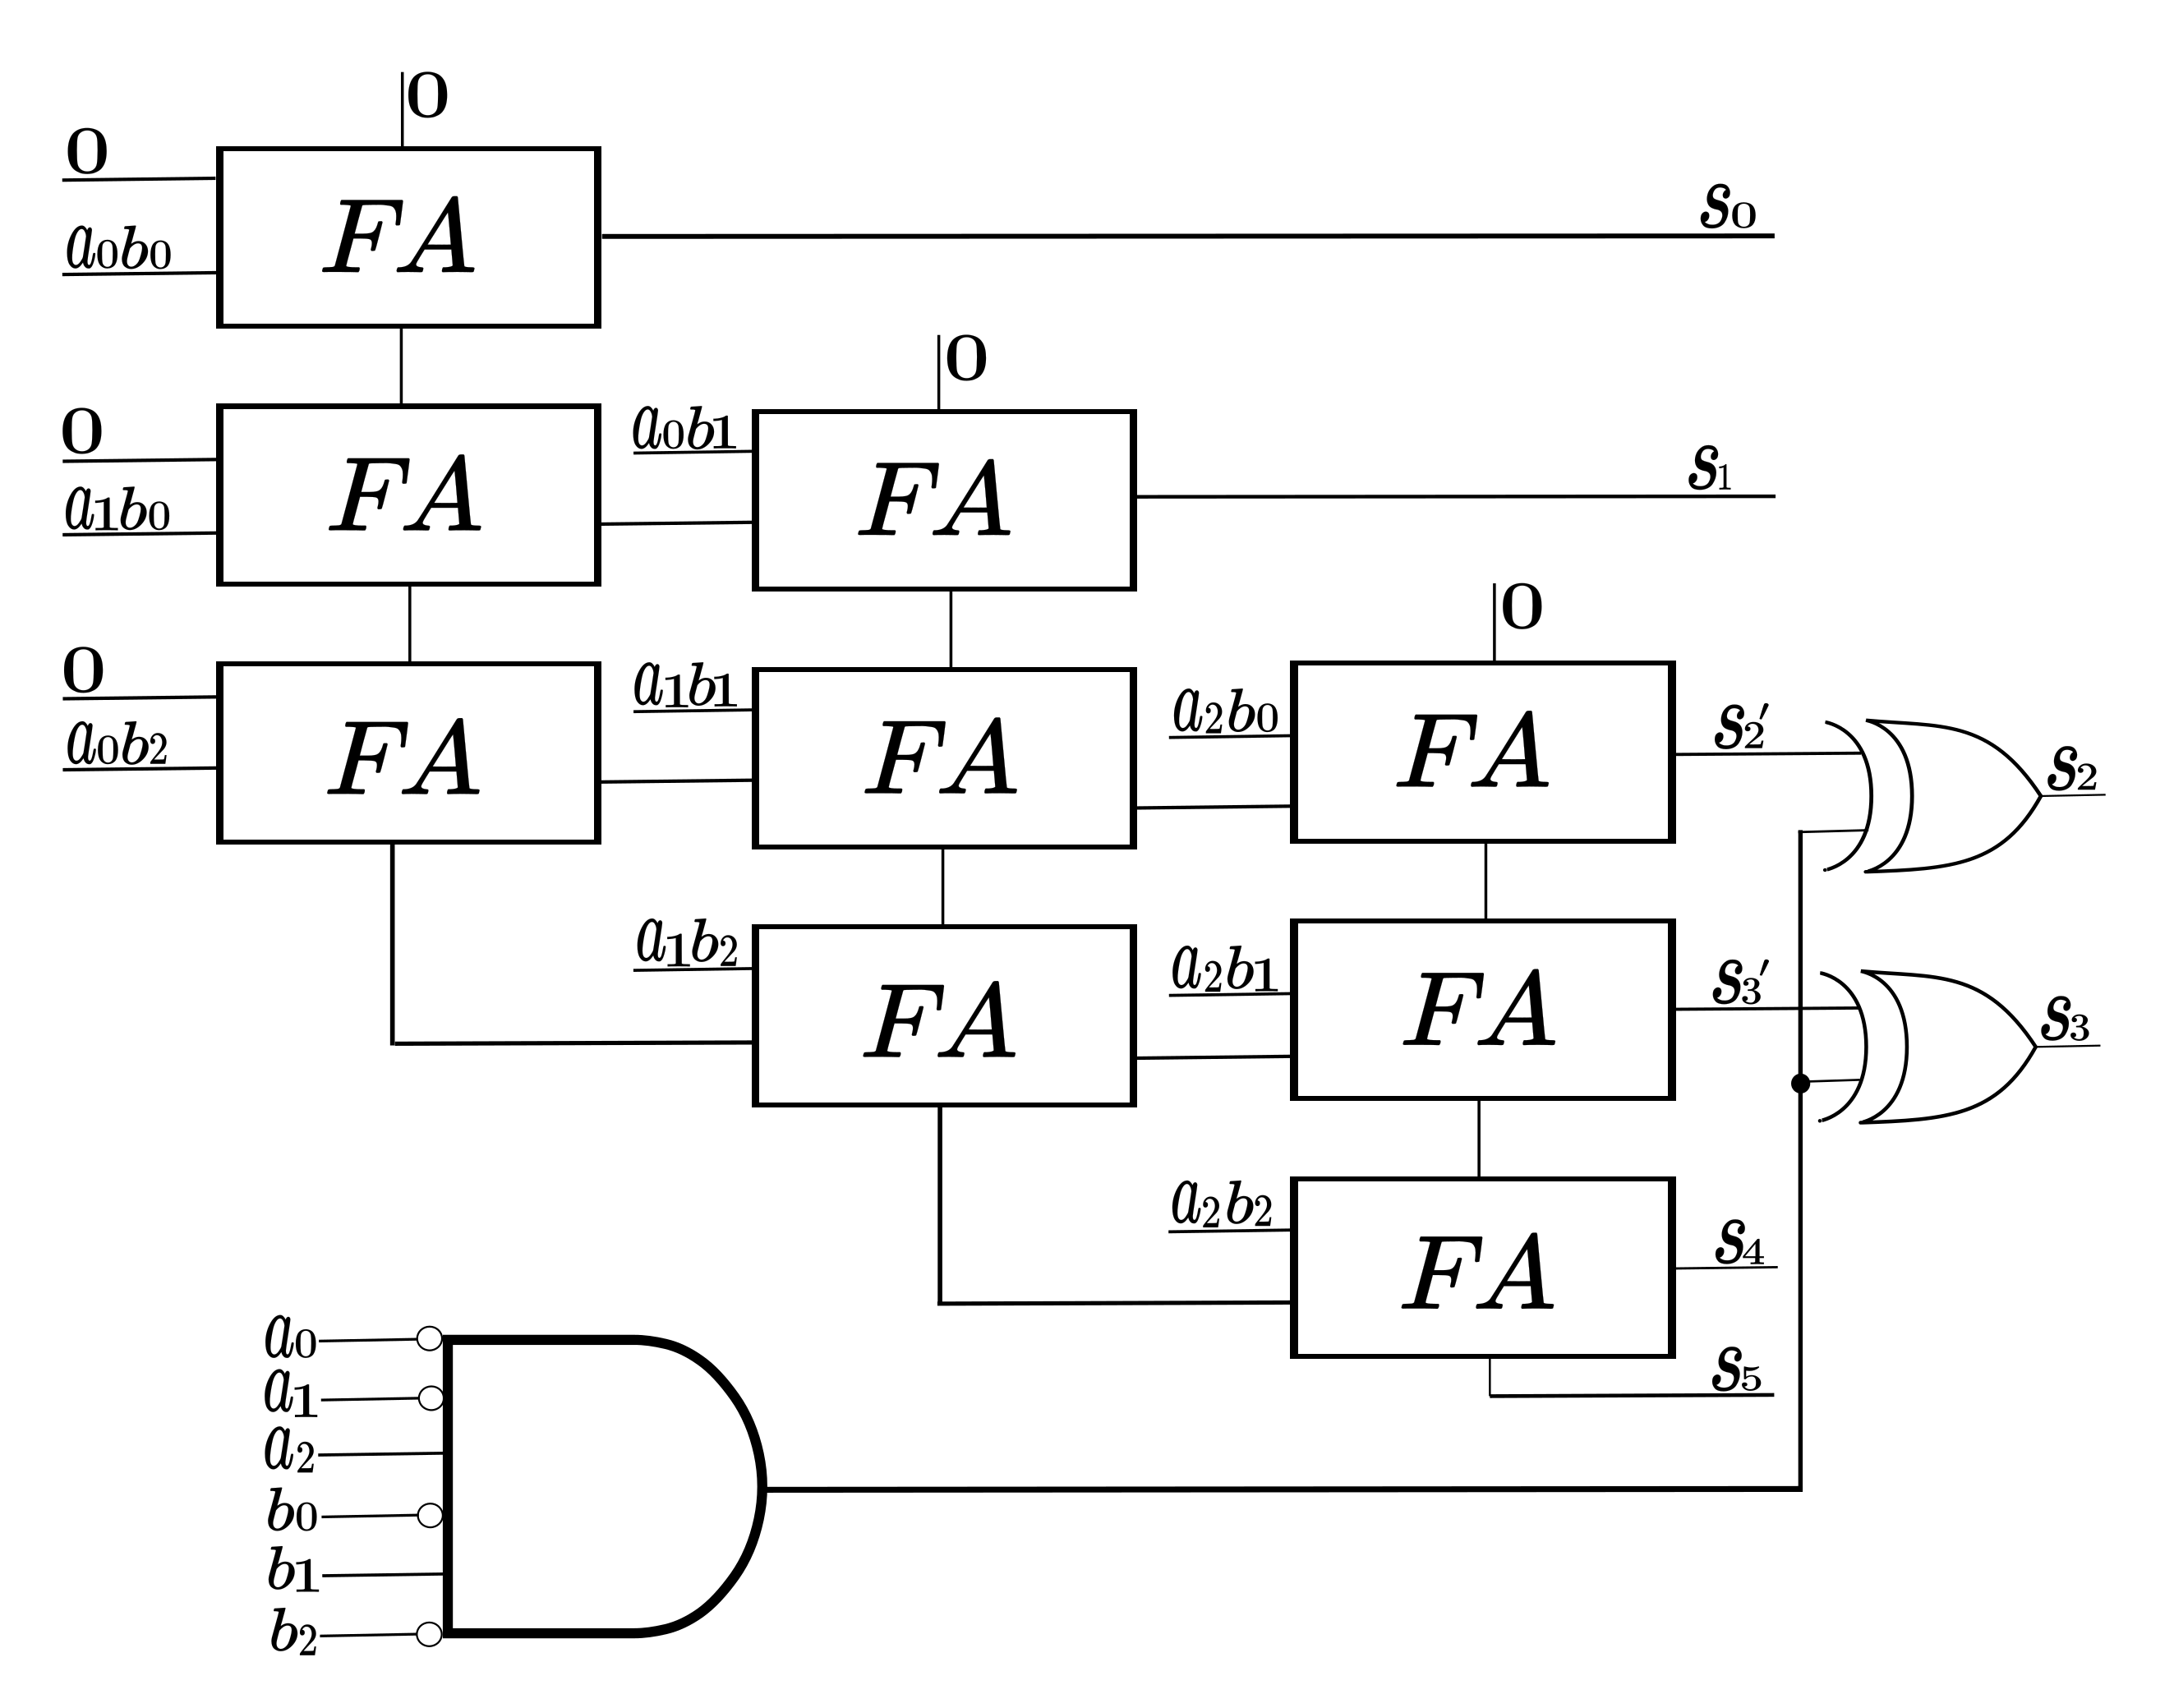
\includegraphics[scale = 0.07]{3appmult.png}
%     \caption{3-bit multiplier with additional circuit to introduce a bug}
%     \label{fig:3appmult}
% \end{figure}

% \end{frame}

% \begin{frame}{\large Research Objective: Integer arithmetic circuits}
% \bi
% 	\item Techniques valid over fields are inapplicable over rings
% 	\item \Grobner basis and division algorithms are complicated
% 	\item Can be modeled over $\Q$
% 	\bi
% 		\item Rectification function computation can result in {\it fractional coefficients}
% 		\item Extracting Boolean rectification function requires exhaustive simulation
% 		\item No scope of optimization as Extended \Grobner basis technique gives zero control
% 	\ei
% \ei

% \end{frame}

% \begin{frame}{\large Research Objective: Integer arithmetic circuits}


% {\tiny
% \begin{equation}
%     \begin{split}
% h_i & = 8\cdot a_0\cdot a_1\cdot a_2\cdot b_0
% +16\cdot a_0\cdot a_1\cdot a_2\cdot b_1
% -12\cdot a_0\cdot a_1 \\
% & -8\cdot a_0\cdot a_2\cdot b_0 
%  -16\cdot a_0\cdot a_2\cdot b_1 
%  +12\cdot a_0-8\cdot a_1\cdot a_2\cdot b_0 \\
% & -16\cdot a_1\cdot a_2\cdot b_1 
% +12\cdot a_1+8\cdot a_2\cdot b_0
% +16\cdot a_2\cdot b_1
% -12        
%     \end{split}
%     \nonumber
% \end{equation}

% \begin{equation}
%     \begin{split}
% h_i' = & -\frac{44}{3}\cdot a_0\cdot a_1\cdot a_2\cdot b_0\cdot b_1\cdot b_2+
% \frac{4}{3}\cdot a_0\cdot a_1\cdot a_2\cdot b_0\cdot b_1 \\
% & +8\cdot a_0\cdot a_1\cdot a_2\cdot b_0\cdot b_2
% +\frac{8}{3}\cdot a_0\cdot a_1\cdot a_2\cdot b_1\cdot b_2 \\
% & +\frac{4}{3} \cdot a_0\cdot a_1\cdot b_0\cdot b_1\cdot b_2
% -\frac{2}{3}\cdot a_0\cdot a_1\cdot b_0\cdot b_1 \\
% &+\frac{4}{3}\cdot a_0\cdot a_1\cdot b_1\cdot b_2
% +\frac{8}{3}\cdot a_0\cdot a_2\cdot b_0\cdot b_1\cdot b_2 \\
% & -4\cdot a_0\cdot a_2\cdot b_0\cdot b_2 
% +\frac{28}{3}\cdot a_1\cdot a_2\cdot b_0\cdot b_1\cdot b_2 \\
% & -\frac{14}{3}\cdot a_1\cdot a_2\cdot b_0\cdot b_1
% -\frac{8}{3}\cdot a_1\cdot a_2\cdot b_0\cdot b_2 \\
% &-\frac{20}{3}\cdot a_1\cdot a_2\cdot b_1\cdot b_2
% +\frac{8}{3}\cdot a_1\cdot a_2\cdot b_1 \\
% &-\frac{2}{3}\cdot a_1\cdot b_1 
% -\frac{4}{3}\cdot a_1\cdot b_2
% +1        
% \end{split}
% \nonumber
% \end{equation}}
% \end{frame}

% \begin{frame}{\large Research Objective: Integer arithmetic circuits}
% \begin{equation*}
%     r = -h_i'h_i+h_{i+1}'f_{i+1}+\dots+h_s'f_s+ \sum H_l' (x_l^2-x_l)
%     \label{eq:eqn6}
% \end{equation*}

% \vspace{2mm}
% \begin{table}[ht]
%     \centering
%     \begin{tabular}{|c|c|c|} \hline
%       $a_0,a_1,a_2,b_0,b_1,b_2$ & $h_i$ & $h_i'$ \\ \hline
%        0,0,0,0,0,0 & -12 & 1\\ \hline
%        0,0,0,0,0,1 & -12 & 1\\ \hline
%        0,0,0,0,1,0 & -12 & 1\\ \hline
%        0,1,0,0,0,1 & 0 & $-\frac{1}{3}$\\ \hline
%        0,1,0,0,1,0 & 0 & $\frac{1}{3}$\\ \hline
%        0,1,0,0,1,1 & 0 & -1 \\ \hline
%     \end{tabular}
%     \caption{Evaluating $h_i$ and $h_i'$}
%     \label{tab:quosol}
% \end{table}

% \bi
% 	\item Challenge: Formulating don't cares
% \ei

% \end{frame}

\begin{frame}{\large Focus: Finite Field Arithmetic Circuits}
\bi
	\item Applications:
	\bi
		\item RSA, ECC, Error correcting codes, RFID, etc.
		\bi
			\item Crypto-system bugs can leak secret keys [{\it Biham. et al}, Crypto'08]
			\item RFID tag cloning could cause counterfeiting [{\it Batina. et al}, Security'09]
		\ei
		\item Large datapath sizes in ECC crypto systems 
		\bi
			\item In $\Fkn$, $n=163, 233, 283, 409, 571$ (NIST standard)
		\ei
	\ei
	\vspace{0.1in}
	\item Rectification Motivation: 
	\bi
		% \item Arithmetic circuits mostly custom designed; potential for errors
		\item Synthesize sub-functions as opposed to complete redesign
		\item Automated debugging
	\ei
\ei
\end{frame}

\begin{frame}{\large MFR Experiments: SINGULAR Implementation}

{\small
\begin{table}[]
\centering
\caption{{\footnotesize Word-level multi-fix rectifiability check against word level specification. Time is in seconds; rows marked '*' indicates $m \nmid n$; Benchmark = Mastrovito architecture, $n$ = Datapath Size, \#Gates = No. of gates, K = $10^3$, $m$ = patch size, $k$ = encompassing composite field size, PF = time for polynomial factorization and computing minpoly for the composite field, RC = time for rectification check}}
\label{masusmontspec}
\begin{tabular}{| c | c | c | c | c | c |} \hline
{\textbf{n}}& {\textbf{\#Gates}} & {\textbf{m}} & {\textbf{k}} & {\textbf{PF}} & {\textbf{RC}} \\ \hline 
12  & 0.45K & 2 & 12  & NA & 0.4\\ \hline
16  & 0.8K & 2 & 16  & NA & 3.2 \\ \hline
*16 & 0.8K & 3 & 48  & -- & --  \\ \hline
*20 & 0.0 & 3 & 60  & -- & --   \\ \hline
32  & 2.8K & 2 & 32  & NA & 184 \\ \hline
48  & 6.4K & 3 & 48  & NA & --  \\ \hline
64  & 11.2K & 2 & 64  & NA & -- \\ \hline
\end{tabular}
\end{table}}

\end{frame}

\begin{frame}{\large MFR Experiments: Custom software}

{\tiny
\begin{table}[]
\centering
\caption{{\footnotesize Word-level multi-fix rectifiability check against word level specification. Time is in seconds; Benchmark = Mastrovito architecture, $n$ = Datapath Size, \#Gates = No. of gates, K = $10^3$, $m$ = word length of patch function, $k$ = encompassing composite field size (degree of primpoly used), PF = time for polynomial factorization and computing minpoly for the composite field, PBS = PolyBori setup (ring declaration/poly collection/spec collection), VF = time for verification, MFS = Multi-fix check setup, MFRC = time for multi-fix rectification check, TE = Total execution time}}
\label{mavsspec}
\begin{tabular}{| c | c | c | c | c | c | c | c | c | c |} \hline
% \multicolumn{6}{| c |}{Benchmark: Mastrovito} & \multicolumn{6}{ c |}{Benchmark: Montgomery} \\ \hline
{\textbf{$n$}} & {\textbf{\#Gates}} & {\textbf{$m$}} & {\textbf{$k$}} & {\textbf{PF}} & {\textbf{PBS}} & {\textbf{$VF$}} & {\textbf{$MFS$}} & {\textbf{$MFRC$}} & {\textbf{$TE$}}\\ \hline 
12   & 0.45K & 2 & 12   & $<$0.01 & $<$0.01 & $<$0.01  & $<$0.01 & $<$0.01 & $<$0.01  \\ \hline
12   & 0.45K & 3 & 12   & $<$0.01 & $<$0.01 & $<$0.01  & $<$0.01 & $<$0.01 & $<$0.01  \\ \hline
16   & 0.8K  & 2 & 16   & $<$0.01 & $<$0.01 & $<$0.01  & $<$0.01 & $<$0.01 & $<$0.01  \\ \hline
16 	 & 0.8K  & 3 & 48   & $<$0.01 & $<$0.01 & $<$0.01  & $<$0.01 & $<$0.01 & $<$0.01  \\ \hline
32   & 2.8K  & 2 & 32   & $<$0.01 & 0.1     & $<$0.01  & $<$0.01 & $<$0.01 & 0.15     \\ \hline
%48   & 6.4K  & 3 & 48  & NA &    &   &  &  &  \\ \hline
64   & 11.2K & 2 & 64   & $<$0.1  & 0.5     & $<$0.01  & $<$0.01 & 0.2     & 0.9      \\ \hline
96   & 24.5K & 2 & 96   & $<$0.1  & 1.4     & 0.1      & $<$0.01 & $<$0.01 & 1.7      \\ \hline
128  & 43.2K & 2 & 128  & $<$0.3  & 3.1     & 0.3      & $<$0.1  & $<$0.1  & 3.6      \\ \hline
163  & 69.8K & 2 & 326  & $<$0.4  & 6.2     & 2.0      & $<$0.1  & 0.4     & 7.5      \\ \hline
233  & 119K  & 2 & 466  & $<$1    & 13.0    & 0.9      & 0.15    & $<$0.1  & 14.3     \\ \hline
283  & 190K  & 2 & 566  & $<$2    & 39.0    & 2.1      & 0.2     & $<$0.1  & 41.3     \\ \hline
409  & 384K  & 2 & 818  & $<$2    & 190     & 3.5      & 0.5     & 0.1     & 195.4    \\ \hline
571  & 827K  & 2 & 1042 & $<$3    & 2170    & 9.1      & 1.1     & $<$0.1  & 2183     \\ \hline

\end{tabular}
\end{table}}
\end{frame}

\begin{frame}{\large Rectification function computation }

\bi
	\item SFR of finite field arithmetic circuits
		[{\it Rao. et al}, FMCAD'18][{\it Rao. et al}, IWLS'18]
	\bi
		\item Quantification based computation
		\item Alternate to Craig Interpolation  
	\ei
\vspace{0.1in}
\item Currently addressing function computation at a word-level for finite field arithmetic circuits: 
\bi
\item Rectification function computation at multiple nets in terms of primary inputs [Due notification GLSVLSI'21]
\bi
	% \item Synthesizing a correction function in terms of primary inputs 
	\item Define and formulate existence of don't cares 
	\item Devise algorithms to explore don't cares for logic optimization 
\ei
\item Formulate rectification setup in terms of internal nets of the circuit. 
\bi
	\item Explore word-level don't care formulation in terms of internal nets.
\ei
\item Extend the multi-fix approach to integer arithmetic circuits and address the associated challenges.
\ei
\ei
\end{frame}

% \begin{frame}{\large Objectives}
% \begin{enumerate}
% 	\item Enhance the investigations on MFR of finite field circuits to accommodate the following challenges 
% 	\vspace{0.1in}
% 	\bi
% 		\item Heuristics to identify effective rectification targets
% 		\vspace{0.1in}
% 		\item Rectification setup in terms of internal nets 
% 		\vspace{0.1in}
% 		\item Derive a word-level abstraction model
% 		\bi
% 			\item Address mathematical challenges posed by the word-level formulation
% 		\ei
% 		\vspace{0.1in}
% 		\item Define and formulate existence of don't cares at the word-level
% 		\vspace{0.1in}
% 		\item Devise algorithms to compute efficient low cost patch functions by exploring the don't care setup 
% 	\ei
% \end{enumerate}
% \end{frame}

% \begin{frame}{\large Objectives}
% \begin{enumerate}
% \setcounter{enumi}{1}
% 	\item Extension to integer arithmetic circuits
% 	\bi
% 		\item Formulate the MFR approach 
% 		\item Address the mathematical challenges associated with it  
% 	\ei
% 	\vspace{0.1in}	
% 	\item Improving scalability of the approach
% 	\bi
% 		\item Utilize PolyBori’s reduction procedure with ZDD data structure
% 		\item Develop a computational engine to implement the rectification framework
% 	\ei
% 	\vspace{0.1in}
% 	\item Theory of permissible functions [{\it Muroga. et al} ITC'89][{\it Fujita. et al} IWLS'19] 
% 	\bi
% 		\item Use don't cares for logic optimization
% 	\ei
% \end{enumerate}
% \end{frame}